% Created by tikzDevice version 0.12.4 on 2023-07-12 07:55:34
% !TEX encoding = UTF-8 Unicode
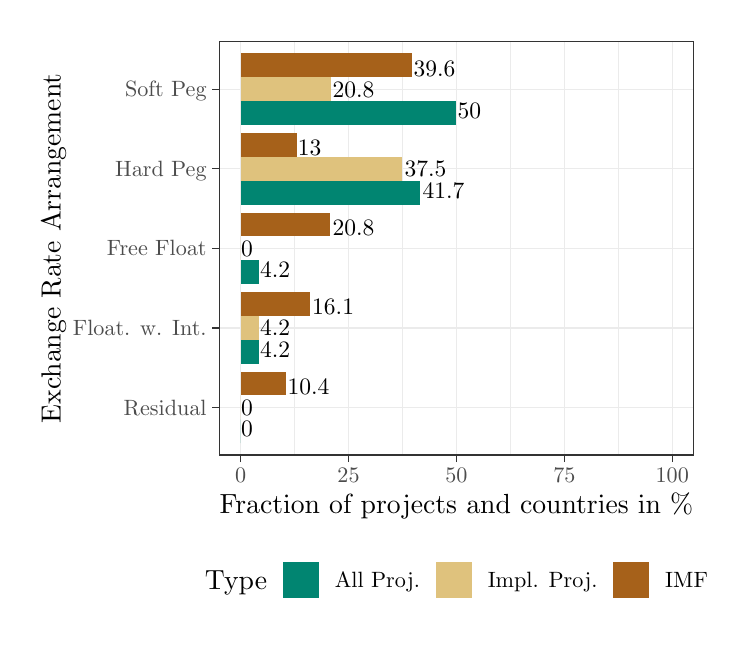
\begin{tikzpicture}[x=1pt,y=1pt]
\definecolor{fillColor}{RGB}{255,255,255}
\path[use as bounding box,fill=fillColor,fill opacity=0.00] (0,0) rectangle (245.72,216.81);
\begin{scope}
\path[clip] (  0.00,  0.00) rectangle (245.72,216.81);
\definecolor{drawColor}{RGB}{255,255,255}
\definecolor{fillColor}{RGB}{255,255,255}

\path[draw=drawColor,line width= 0.5pt,line join=round,line cap=round,fill=fillColor] (  0.00,  0.00) rectangle (245.72,216.81);
\end{scope}
\begin{scope}
\path[clip] ( 69.15, 62.35) rectangle (240.72,211.81);
\definecolor{fillColor}{RGB}{255,255,255}

\path[fill=fillColor] ( 69.15, 62.35) rectangle (240.72,211.81);
\definecolor{drawColor}{gray}{0.92}

\path[draw=drawColor,line width= 0.3pt,line join=round] ( 96.45, 62.35) --
	( 96.45,211.81);

\path[draw=drawColor,line width= 0.3pt,line join=round] (135.44, 62.35) --
	(135.44,211.81);

\path[draw=drawColor,line width= 0.3pt,line join=round] (174.43, 62.35) --
	(174.43,211.81);

\path[draw=drawColor,line width= 0.3pt,line join=round] (213.42, 62.35) --
	(213.42,211.81);

\path[draw=drawColor,line width= 0.5pt,line join=round] ( 69.15, 79.60) --
	(240.72, 79.60);

\path[draw=drawColor,line width= 0.5pt,line join=round] ( 69.15,108.34) --
	(240.72,108.34);

\path[draw=drawColor,line width= 0.5pt,line join=round] ( 69.15,137.08) --
	(240.72,137.08);

\path[draw=drawColor,line width= 0.5pt,line join=round] ( 69.15,165.82) --
	(240.72,165.82);

\path[draw=drawColor,line width= 0.5pt,line join=round] ( 69.15,194.56) --
	(240.72,194.56);

\path[draw=drawColor,line width= 0.5pt,line join=round] ( 76.95, 62.35) --
	( 76.95,211.81);

\path[draw=drawColor,line width= 0.5pt,line join=round] (115.94, 62.35) --
	(115.94,211.81);

\path[draw=drawColor,line width= 0.5pt,line join=round] (154.94, 62.35) --
	(154.94,211.81);

\path[draw=drawColor,line width= 0.5pt,line join=round] (193.93, 62.35) --
	(193.93,211.81);

\path[draw=drawColor,line width= 0.5pt,line join=round] (232.92, 62.35) --
	(232.92,211.81);
\definecolor{fillColor}{RGB}{1,133,113}

\path[fill=fillColor] ( 76.95,152.89) rectangle (141.94,161.51);

\path[fill=fillColor] ( 76.95,181.63) rectangle (154.94,190.25);

\path[fill=fillColor] ( 76.95,124.15) rectangle ( 83.45,132.77);

\path[fill=fillColor] ( 76.95, 95.40) rectangle ( 83.45,104.03);

\path[fill=fillColor] ( 76.95, 66.66) rectangle ( 76.95, 75.28);
\definecolor{fillColor}{RGB}{223,194,125}

\path[fill=fillColor] ( 76.95,161.51) rectangle (135.44,170.13);

\path[fill=fillColor] ( 76.95,190.25) rectangle (109.44,198.88);

\path[fill=fillColor] ( 76.95,132.77) rectangle ( 76.95,141.39);

\path[fill=fillColor] ( 76.95,104.03) rectangle ( 83.45,112.65);

\path[fill=fillColor] ( 76.95, 75.28) rectangle ( 76.95, 83.91);
\definecolor{fillColor}{RGB}{166,97,26}

\path[fill=fillColor] ( 76.95,170.13) rectangle ( 97.23,178.76);

\path[fill=fillColor] ( 76.95,198.88) rectangle (138.71,207.50);

\path[fill=fillColor] ( 76.95,141.39) rectangle (109.39,150.01);

\path[fill=fillColor] ( 76.95,112.65) rectangle (102.06,121.27);

\path[fill=fillColor] ( 76.95, 83.91) rectangle ( 93.17, 92.53);
\definecolor{drawColor}{RGB}{0,0,0}

\node[text=drawColor,anchor=base west,inner sep=0pt, outer sep=0pt, scale=  0.85] at (142.70,155.22) {41.7};

\node[text=drawColor,anchor=base west,inner sep=0pt, outer sep=0pt, scale=  0.85] at (155.36,183.96) {50};

\node[text=drawColor,anchor=base west,inner sep=0pt, outer sep=0pt, scale=  0.85] at ( 84.00,126.48) {4.2};

\node[text=drawColor,anchor=base west,inner sep=0pt, outer sep=0pt, scale=  0.85] at ( 84.00, 97.73) {4.2};

\node[text=drawColor,anchor=base west,inner sep=0pt, outer sep=0pt, scale=  0.85] at ( 77.16, 68.99) {0};

\node[text=drawColor,anchor=base west,inner sep=0pt, outer sep=0pt, scale=  0.85] at (136.20,162.88) {37.5};

\node[text=drawColor,anchor=base west,inner sep=0pt, outer sep=0pt, scale=  0.85] at (110.20,191.63) {20.8};

\node[text=drawColor,anchor=base west,inner sep=0pt, outer sep=0pt, scale=  0.85] at ( 77.16,134.14) {0};

\node[text=drawColor,anchor=base west,inner sep=0pt, outer sep=0pt, scale=  0.85] at ( 84.00,105.40) {4.2};

\node[text=drawColor,anchor=base west,inner sep=0pt, outer sep=0pt, scale=  0.85] at ( 77.16, 76.66) {0};

\node[text=drawColor,anchor=base west,inner sep=0pt, outer sep=0pt, scale=  0.85] at ( 97.65,170.55) {13};

\node[text=drawColor,anchor=base west,inner sep=0pt, outer sep=0pt, scale=  0.85] at (139.47,199.29) {39.6};

\node[text=drawColor,anchor=base west,inner sep=0pt, outer sep=0pt, scale=  0.85] at (110.15,141.81) {20.8};

\node[text=drawColor,anchor=base west,inner sep=0pt, outer sep=0pt, scale=  0.85] at (102.82,113.06) {16.1};

\node[text=drawColor,anchor=base west,inner sep=0pt, outer sep=0pt, scale=  0.85] at ( 93.93, 84.32) {10.4};
\definecolor{drawColor}{gray}{0.20}

\path[draw=drawColor,line width= 0.5pt,line join=round,line cap=round] ( 69.15, 62.35) rectangle (240.72,211.81);
\end{scope}
\begin{scope}
\path[clip] (  0.00,  0.00) rectangle (245.72,216.81);
\definecolor{drawColor}{gray}{0.30}

\node[text=drawColor,anchor=base east,inner sep=0pt, outer sep=0pt, scale=  0.80] at ( 64.65, 76.84) {Residual};

\node[text=drawColor,anchor=base east,inner sep=0pt, outer sep=0pt, scale=  0.80] at ( 64.65,105.58) {Float. w. Int.};

\node[text=drawColor,anchor=base east,inner sep=0pt, outer sep=0pt, scale=  0.80] at ( 64.65,134.33) {Free Float};

\node[text=drawColor,anchor=base east,inner sep=0pt, outer sep=0pt, scale=  0.80] at ( 64.65,163.07) {Hard Peg};

\node[text=drawColor,anchor=base east,inner sep=0pt, outer sep=0pt, scale=  0.80] at ( 64.65,191.81) {Soft Peg};
\end{scope}
\begin{scope}
\path[clip] (  0.00,  0.00) rectangle (245.72,216.81);
\definecolor{drawColor}{gray}{0.20}

\path[draw=drawColor,line width= 0.5pt,line join=round] ( 66.65, 79.60) --
	( 69.15, 79.60);

\path[draw=drawColor,line width= 0.5pt,line join=round] ( 66.65,108.34) --
	( 69.15,108.34);

\path[draw=drawColor,line width= 0.5pt,line join=round] ( 66.65,137.08) --
	( 69.15,137.08);

\path[draw=drawColor,line width= 0.5pt,line join=round] ( 66.65,165.82) --
	( 69.15,165.82);

\path[draw=drawColor,line width= 0.5pt,line join=round] ( 66.65,194.56) --
	( 69.15,194.56);
\end{scope}
\begin{scope}
\path[clip] (  0.00,  0.00) rectangle (245.72,216.81);
\definecolor{drawColor}{gray}{0.20}

\path[draw=drawColor,line width= 0.5pt,line join=round] ( 76.95, 59.85) --
	( 76.95, 62.35);

\path[draw=drawColor,line width= 0.5pt,line join=round] (115.94, 59.85) --
	(115.94, 62.35);

\path[draw=drawColor,line width= 0.5pt,line join=round] (154.94, 59.85) --
	(154.94, 62.35);

\path[draw=drawColor,line width= 0.5pt,line join=round] (193.93, 59.85) --
	(193.93, 62.35);

\path[draw=drawColor,line width= 0.5pt,line join=round] (232.92, 59.85) --
	(232.92, 62.35);
\end{scope}
\begin{scope}
\path[clip] (  0.00,  0.00) rectangle (245.72,216.81);
\definecolor{drawColor}{gray}{0.30}

\node[text=drawColor,anchor=base,inner sep=0pt, outer sep=0pt, scale=  0.80] at ( 76.95, 52.34) {0};

\node[text=drawColor,anchor=base,inner sep=0pt, outer sep=0pt, scale=  0.80] at (115.94, 52.34) {25};

\node[text=drawColor,anchor=base,inner sep=0pt, outer sep=0pt, scale=  0.80] at (154.94, 52.34) {50};

\node[text=drawColor,anchor=base,inner sep=0pt, outer sep=0pt, scale=  0.80] at (193.93, 52.34) {75};

\node[text=drawColor,anchor=base,inner sep=0pt, outer sep=0pt, scale=  0.80] at (232.92, 52.34) {100};
\end{scope}
\begin{scope}
\path[clip] (  0.00,  0.00) rectangle (245.72,216.81);
\definecolor{drawColor}{RGB}{0,0,0}

\node[text=drawColor,anchor=base,inner sep=0pt, outer sep=0pt, scale=  1.00] at (154.94, 41.40) {Fraction of projects and countries in \%};
\end{scope}
\begin{scope}
\path[clip] (  0.00,  0.00) rectangle (245.72,216.81);
\definecolor{drawColor}{RGB}{0,0,0}

\node[text=drawColor,rotate= 90.00,anchor=base,inner sep=0pt, outer sep=0pt, scale=  1.00] at ( 11.89,137.08) {Exchange Rate Arrangement};
\end{scope}
\begin{scope}
\path[clip] (  0.00,  0.00) rectangle (245.72,216.81);
\definecolor{fillColor}{RGB}{255,255,255}

\path[fill=fillColor] ( 59.05,  5.00) rectangle (250.82, 29.45);
\end{scope}
\begin{scope}
\path[clip] (  0.00,  0.00) rectangle (245.72,216.81);
\definecolor{drawColor}{RGB}{0,0,0}

\node[text=drawColor,anchor=base west,inner sep=0pt, outer sep=0pt, scale=  1.00] at ( 64.05, 13.78) {Type};
\end{scope}
\begin{scope}
\path[clip] (  0.00,  0.00) rectangle (245.72,216.81);
\definecolor{fillColor}{RGB}{255,255,255}

\path[fill=fillColor] ( 91.55, 10.00) rectangle (106.00, 24.45);
\end{scope}
\begin{scope}
\path[clip] (  0.00,  0.00) rectangle (245.72,216.81);
\definecolor{fillColor}{RGB}{1,133,113}

\path[fill=fillColor] ( 92.26, 10.71) rectangle (105.29, 23.74);
\end{scope}
\begin{scope}
\path[clip] (  0.00,  0.00) rectangle (245.72,216.81);
\definecolor{fillColor}{RGB}{255,255,255}

\path[fill=fillColor] (146.79, 10.00) rectangle (161.25, 24.45);
\end{scope}
\begin{scope}
\path[clip] (  0.00,  0.00) rectangle (245.72,216.81);
\definecolor{fillColor}{RGB}{223,194,125}

\path[fill=fillColor] (147.50, 10.71) rectangle (160.53, 23.74);
\end{scope}
\begin{scope}
\path[clip] (  0.00,  0.00) rectangle (245.72,216.81);
\definecolor{fillColor}{RGB}{255,255,255}

\path[fill=fillColor] (210.93, 10.00) rectangle (225.38, 24.45);
\end{scope}
\begin{scope}
\path[clip] (  0.00,  0.00) rectangle (245.72,216.81);
\definecolor{fillColor}{RGB}{166,97,26}

\path[fill=fillColor] (211.64, 10.71) rectangle (224.67, 23.74);
\end{scope}
\begin{scope}
\path[clip] (  0.00,  0.00) rectangle (245.72,216.81);
\definecolor{drawColor}{RGB}{0,0,0}

\node[text=drawColor,anchor=base west,inner sep=0pt, outer sep=0pt, scale=  0.80] at (111.00, 14.47) {All Proj.};
\end{scope}
\begin{scope}
\path[clip] (  0.00,  0.00) rectangle (245.72,216.81);
\definecolor{drawColor}{RGB}{0,0,0}

\node[text=drawColor,anchor=base west,inner sep=0pt, outer sep=0pt, scale=  0.80] at (166.25, 14.47) {Impl. Proj.};
\end{scope}
\begin{scope}
\path[clip] (  0.00,  0.00) rectangle (245.72,216.81);
\definecolor{drawColor}{RGB}{0,0,0}

\node[text=drawColor,anchor=base west,inner sep=0pt, outer sep=0pt, scale=  0.80] at (230.38, 14.47) {IMF};
\end{scope}
\end{tikzpicture}
